% =====================================================================
% SEÇÃO 3 — METODOLOGIA
% Estrutura inspirada em:
%   - da Silva, Rodrigues-Jr & de Albuquerque (2025), "On the power of CNNs
%     to detect slums in Brazil", Computers, Environment and Urban Systems
%     (estágios numerados: aquisição -> processamento -> treino -> análise)
%   - Soliani et al. (2024), "Catastrophic causes of truck drivers' crashes
%     on Brazilian highways", Multimodal Transportation
%     (bloco explicativo/causal primeiro, bloco preditivo depois)
% =====================================================================

\section{Metodologia}

A metodologia está organizada em dois blocos, seguindo a lógica adotada
por Soliani et al. \cite{soliani2024} ao investigar acidentes com
caminhões em rodovias brasileiras: um bloco explicativo, que estabelece se
e como o calendário de jogos se associa aos desfechos de interesse, e um
bloco preditivo, que usa essa base para construir e validar modelos de
previsão de picos. A Figura~\ref{fig:pipeline} resume as quatro etapas do
pipeline -- integração de dados, análise exploratória e causal, definição
do alvo e engenharia de atributos, e modelagem preditiva --, no espírito
do diagrama de estágios de da Silva et al. \cite{dasilva2025}.

\begin{figure}[ht]
\centering
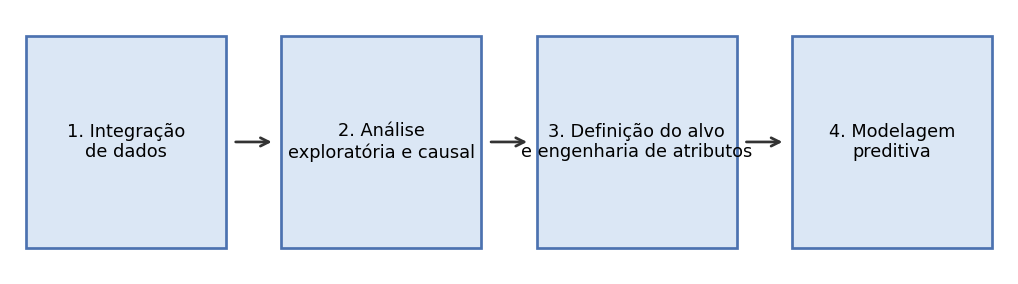
\includegraphics[width=.95\linewidth]{figuras/pipeline.png}
\caption{Etapas do pipeline de dados e análise}
\label{fig:pipeline}
\end{figure}

\subsection{Fontes de dados e integração}

Quatro categorias de dados públicos foram integradas para o município de
São Paulo, no período de 2022-01-01 a 2023-12-31 (730 dias, a janela de
sobreposição entre as três fontes principais):

\begin{itemize}
\item \textbf{Criminalidade} -- SPDadosCriminais (SSP-SP), microdados de
  boletim de ocorrência (grão real é BO$\times$rubrica, não BO único),
  filtrados por código IBGE do município (3550308, mais confiável que o
  campo textual da cidade, que tem variantes de grafia/espaço em branco);
\item \textbf{Sinistros de trânsito} -- Infosiga SP (Detran-SP), mesmo
  filtro geográfico, granularidade de evento, \emph{encoding} latin-1;
\item \textbf{Partidas de futebol} -- base histórica do Campeonato
  Brasileiro (Séries A/B/C) e Copa do Brasil (2014--2023), restrita aos
  mandantes que jogam na capital (Corinthians, Palmeiras e São Paulo FC --
  o Santos manda em Santos-SP, fora do escopo como mandante); clássico
  definido como mandante \emph{e} visitante pertencentes a
  \{Corinthians, Palmeiras, São Paulo, Santos\};
\item \textbf{Clima e calendário} -- estação INMET A701 (Mirante),
  agregada de horária (UTC) para diária (Brasília, $-3$h fixo, sem
  horário de verão), mais feriados (calculados por algoritmo de Páscoa,
  sem depender de API externa) e calendário escolar da rede municipal
  (transcrito manualmente de resoluções oficiais).
\end{itemize}

Cada fonte foi agregada ao grão \emph{dia} e unida por uma chave de
calendário mestre, garantindo que dias sem jogo, chuva ou ocorrência
apareçam com valor zero explícito, não como linha ausente. Dois cuidados
de qualidade afetam diretamente a validade das análises subsequentes:
os últimos dois dias da série (30--31/12/2023) têm contagens anormalmente
baixas por defasagem no registro administrativo, não queda real, e foram
excluídos de todos os testes e treinamentos; e um dia isolado
(19/06/2022) tem um pico de furtos compatível com lançamento retroativo em
lote, cujo tratamento foi avaliado por análise de sensibilidade.

\subsection{Bloco explicativo: associação entre jogos e desfechos}

Antes de qualquer modelo preditivo, testou-se se dias de jogo se associam
a desfechos elevados de criminalidade e sinistros, e se essa associação
sobrevive ao controle por calendário -- réplica do cuidado de Soliani et
al. \cite{soliani2024} em separar a análise de causas da etapa preditiva.

\textbf{Comparação bruta e ajustada.} Dias com e sem jogo foram comparados
por Mann–Whitney (distribuição não-normal confirmada previamente), com
correção de Benjamini--Hochberg \cite{bh1995} para múltiplas comparações,
e reestimados por Modelo Linear Generalizado Poisson com erros-padrão
robustos (HC1),

\begin{equation}
\log(\mathrm{E}[y_d]) = \beta_0 + \beta_1\,\text{jogo}_d +
  \gamma\,\text{diaSemana}_d + \delta\,\text{mês}_d + \epsilon\,\text{feriado}_d,
\end{equation}

controlando por dia da semana e mês -- este último necessário porque a
temporada de futebol (abril--novembro) não cobre o verão
(dezembro--março), o que poderia confundir efeito de jogo com sazonal.

\textbf{Defasagem temporal.} Um modelo de defasagens distribuídas
($\text{jogo}_{d-2}\ldots\text{jogo}_{d+2}$) e uma correlação cruzada
sobre séries dessazonalizadas (resíduo de
$\text{OLS}(y \sim \text{diaSemana} + \text{mês} + \text{feriado})$)
avaliaram se o efeito, caso exista, precede ou sucede o jogo.

\textbf{Causalidade formal.} Aplicou-se pareamento por escore de
propensão (\emph{Propensity Score Matching}, vizinho mais próximo,
\emph{caliper} de 0,2 desvio-padrão do logit do escore, seguindo Austin
\cite{austin2011}) e ponderação por probabilidade inversa de tratamento
(IPTW) como robustez, além de uma adaptação de \emph{Interrupted Time
Series} em torno do evento de maior público da base. A violação de
positividade (ausência de jogos em janeiro--fevereiro) foi verificada
explicitamente antes do pareamento.

\subsection{Definição da variável-alvo}

Em vez de um limiar arbitrário sobre a contagem bruta — que se mostrou
equivalente, na prática, a um classificador de fim de semana —, o alvo de
"pico" foi definido sobre o resíduo dessazonalizado: um dia é considerado
pico quando esse resíduo excede o percentil 90 da sua distribuição
histórica. Z-score e média móvel causal (28 dias) foram mantidos como
variantes de robustez, seguindo a recomendação de testar múltiplas
formulações antes de fixar uma definição única.

\subsection{Bloco preditivo: engenharia de atributos e modelos}

\textbf{Atributos.} A tabela analítica final tem 730 linhas $\times$ 95
atributos (mais 10 variantes de alvo), organizados em quatro grupos:
temporais (26, todos conhecidos com antecedência: calendário,
sazonalidade); de futebol (20, mandante, clássico, horário --resultado e
gols do próprio jogo excluídos por vazamento de informação, e
público/taxa de ocupação bloqueados por ausência total da variável);
climáticos (11, previsão do dia mais uma variante conservadora defasada
em 1 dia); e históricos (38, defasagens de 1, 2, 3, 7, 14, 28 e 364 dias e
médias móveis de 7/14/28 dias do próprio desfecho, sempre com
deslocamento mínimo de 1 dia, auditado automaticamente contra
vazamento).

\textbf{Modelos e validação.} Seguindo o cuidado de comparação contra
baseline de Soliani et al. \cite{soliani2024}, testaram-se baselines
(média histórica, média móvel, mesmo dia da semana anterior) contra
Decision Tree, Random Forest, XGBoost \cite{chen2016} e LightGBM
(regressão com perda de Poisson) e Regressão Logística (classificação).
A validação usou janela expansiva com 12 \emph{folds} mensais
(\emph{walk-forward}), nunca divisão aleatória, com o limiar de pico e o
ajuste de calendário reestimados exclusivamente sobre o treino de cada
\emph{fold}, para impedir vazamento do teste.

\textbf{Otimização e interpretabilidade.} A busca de hiperparâmetros usou
validação aninhada (\emph{nested walk-forward}): o nível externo replica
os 12 \emph{folds}, o interno usa \texttt{TimeSeriesSplit} dentro do
treino de cada \emph{fold} externo. A contribuição de cada grupo de
atributos foi quantificada por valores de Shapley (SHAP)
\cite{lundberg2017}, com \texttt{TreeExplainer} para os modelos de árvore
e explicador linear para a regressão logística; atributos de contribuição
elevada foram auditados quanto à colinearidade com calendário antes de
serem atribuídos a um efeito de futebol -- necessário porque a contagem de
dias até o próximo jogo mostrou-se, neste estudo, proxy quase perfeito de
época do ano.

\textbf{Cenários.} Simulações (ex.: domingo com clássico, quarta-feira com
jogo noturno) foram construídas a partir de dias reais que satisfazem cada
descrição, não de vetores sintéticos, e a diferença entre cada cenário e
sua referência foi decomposta por grupo de atributos via aditividade do
SHAP.
